\documentclass[12pt]{article}



% A package for setting layout and margins for your thesis 
\usepackage[a4paper]{geometry}
\usepackage{float}

% Use package babel for English or Estonian 
% If you use Estonian make sure that Estonian hyphenation is installed 
% - hypen-estonian or eehyp packages
\usepackage[estonian, english]{babel} 
% \usepackage[english]{babel}
% \usepackage[estonian]{babel}
%
%
% When you write in Estonian then you want to use text with right character set
% By default LaTeX does not know what to do with õäöu letters. You have to specify
% a correct input and font encoding. For that you have to Google the Web     
%
% For TexShop under MacOS X. The right lines are 
%\usepackage[applemac]{inputenc}
\usepackage[T1]{fontenc}
%
% For Windows and Linux the right magic lines are   
% \usepackage[latin1]{inputenc}
% \usepackage[latin5]{inputenc}
% \usepackage[T1]{fontenc}


% General packages for math in general, theorems and symbols 
% Read ftp://ftp.ams.org/ams/doc/amsmath/short-math-guide.pdf for further information
\usepackage{amsmath} 
\usepackage{amsthm}
\usepackage{amssymb}

% Optional calligraphic fonts    
% \usepackage[mathscr]{eucal}

% Packages for building tables and tabulars 
\usepackage{array}
\usepackage{tabu}   % Wide lines in tables
\usepackage{xspace} % Non-eatable spaces in macros

% Including graphical images and setting the figure directory
\usepackage{graphicx}
\graphicspath{{figures/}}

% Packages for getting clickable links in PDF file
\usepackage{hyperref}
\usepackage[all]{hypcap}


% Packages for defining colourful text together with some colours
\usepackage{color}
\usepackage{xcolor} 
%\definecolor{dkgreen}{rgb}{0,0.6,0}
%\definecolor{gray}{rgb}{0.5,0.5,0.5}
\definecolor{mauve}{rgb}{0.58,0,0.82}


% Standard package for drawing algorithms
% Since the thesis in article format we must define \chapter for
% the package algorithm2e (otherwise obscure errors occur) 
\let\chapter\section
\usepackage[ruled, vlined, linesnumbered]{algorithm2e}

% Fix a  set of keywords which you use inside algorithms
\SetKw{True}{true}
\SetKw{False}{false}
\SetKwData{typeInt}{Int}
\SetKwData{typeRat}{Rat}
\SetKwData{Defined}{Defined}
\SetKwFunction{parseStatement}{parseStatement}


% Nice todo notes
\usepackage{todonotes}


% Proper way to create coloured code listings
\usepackage{listings}
\lstset{ 
  %language=python,                % the language of the code
  language=C++,
  basicstyle=\footnotesize,        % the size of the fonts that are used for the code
  %numbers=left,                   % where to put the line-numbers
  %numberstyle=\footnotesize,      % the size of the fonts that are used for the line-numbers
  numberstyle=\tiny\color{gray}, 
  stepnumber=1,                    % the step between two line-numbers. If it's 1, each line 
                                   % will be numbered
  numbersep=5pt,                   % how far the line-numbers are from the code
  backgroundcolor=\color{white},   % choose the background color. You must add \usepackage{color}
  showspaces=false,                % show spaces adding particular underscores
  showstringspaces=false,          % underline spaces within strings
  showtabs=false,                  % show tabs within strings adding particular underscores
  frame = lines,
  %frame=single,                   % adds a frame around the code
  rulecolor=\color{black},		   % if not set, the frame-color may be changed on line-breaks within 
                                   % not-black text (e.g. commens (green here))
  tabsize=2,                       % sets default tabsize to 2 spaces
  captionpos=b,                    % sets the caption-position to bottom
  breaklines=true,                 % sets automatic line breaking
  breakatwhitespace=false,         % sets if automatic breaks should only happen at whitespace
  %title=\lstname,                 % show the filename of files included with \lstinputlisting;
                                   % also try caption instead of title
                                   % also try caption instead of title
  keywordstyle=\color{blue},       % keyword style
  commentstyle=\color{dkgreen},    % comment style
  stringstyle=\color{mauve},       % string literal style
  escapeinside={\%*}{*)},          % if you want to add a comment within your code
  morekeywords={*,game, fun}       % if you want to add more keywords to the set
}


% Obscure packages to write logic formulae and program semantics
% Unless you do a bachelor thesis on program semantics or static code analysis you do not need that
% http://logicmatters.net/resources/ndexamples/proofsty3.html <= writing type rules => use semantic::inference
% ftp://tug.ctan.org/tex-archive/macros/latex/contrib/semantic/semantic.pdf
\usepackage{proof}
\usepackage{semantic} 
\setlength{\inferLineSkip}{4pt}
\def\predicatebegin #1\predicateend{$\Gamma \vdash #1$}

% If you really want to draw figures in LaTeX use packages tikz or pstricks
% However, getting a corresponding illustrations is really painful  


% Define your favorite macros that you use inside the thesis 
% Name followed by non-removable space
\newcommand{\proveit}{ProveIt\xspace}

% Macros that make sure that the math mode is set
\newcommand{\typeF}[1] {\ensuremath{\mathsf{type_{#1}}}\xspace}
\newcommand{\opDiv}{\ensuremath{\backslash \mathsf{div}}\xspace} 

% Nice Todo box
\newcommand{\TODO}{\todo[inline]}

% A way to define theorems and lemmata
\newtheorem{theorem}{Theorem}








%%% BEGIN DOCUMENT
\begin{document}

% BEGIN TITLE PAGE
\thispagestyle{empty}
\begin{center}

\large
UNIVERSITY OF TARTU\\[2mm]
Institute of Computer Science\\
Computer Science Curriculum\\[2mm]

%\vspace*{\stretch{5}}
\vspace{25mm}

\Large Jevgeni Savostkin

\vspace{4mm}

\huge Improving accuracy of brain-computer interface with multiple trials

%\vspace*{\stretch{7}}
\vspace{20mm}

\Large Master's Thesis (30 ECTS)

\end{center}

\vspace{2mm}

\begin{flushright}
 {
 \setlength{\extrarowheight}{5pt}
 \begin{tabular}{r l} 
  \sffamily Supervisor: & \sffamily Ilya Kuzovkin, MSc \\ 
  \sffamily Supervisor: & \sffamily Raul Vicente, PhD 
 \end{tabular}
 }
\end{flushright}

%\vspace*{\stretch{3}}
\vspace{10mm}

%{\noindent Author: .................................................................................... ``.....'' ..........\hskip16pt 2048}
\vspace{2mm}


%{\noindent Supervisor: ............................................................................... ``.....'' ..........\hskip16pt 2048}

\vspace{2mm}

%{\noindent Supervisor: ............................................................................... ``.....'' ..........\hskip16pt 2048}

\vspace{8mm}


\vfill
\centerline{Tartu 2017}

% END TITLE PAGE

% If the thesis is printed on both sides of the page then 
% the second page must be must be empty. Comment this out
% if you print only to one side of the page comment this out
% \newpage
% \thispagestyle{empty}    
% \phantom{Text to fill the page}
% END OF EXTRA PAGE WITHOUT NUMBER

\newpage
\selectlanguage{english}
\noindent\textbf{\large Improving accuracy of brain-computer interface with multiple trials}
\vspace*{2ex}
{\flushleft{\textbf{Abstract:}} }

Brain-computer interface (BCI) is a computer system for extracting brain electronic neural signals and using them to control computer applications. Besides measuring, BCI converts raw signals to digital data and maps the data to the exact computer commands. Unfortunately, the probability of the right command prediction usually is below 100\% and therefore it could be improved.

This is a problem for BCI systems, since they will not be widely trusted and used, while the prediction accuracy is relatively low. There are many existing solutions, which provide increase of the prediction accuracy, mainly based on trying out different classification techniques and algorithms. Existing methods focus mostly on a training part of the system. Our approach is to try to improve the accuracy upto 99.9\%, while experimenting with test part algorithms, and to determine how many trials are required during the test mode to reach the desired provided accuracy.

The solution described in the thesis is based on Condorcet's jury theorem. It means that if we have single events with probability of more than 50\%, then by combining them, the total probability for these events would rise. This work shows the actual results (prediction accuracies) and provides their comparison using the voting techniques based on the Condorcet's jury theorem. It also describes the dependency of the number of test mode measurements and accuracies.

The BCI technology is relatively young direction. In order to fully integrate it into our ordinary life, the contribution from the scientist and engineers is required for composing and choosing the most reliable system with the components. The following work represents a contribution to the brain-computer interface field.


\vspace*{3ex}
{\flushleft{\textbf{Keywords:}}}
Brain-computer interface, Random Forests
\vspace*{3ex}

%\noindent\textbf{CERCS:}\TODO{CERCS code and name:~\url{https://www.etis.ee/Portal/Classifiers/Details/d3717f7b-bec8-4cd9-8ea4-c89cd56ca46e}}

\selectlanguage{english}

\newpage
\tableofcontents

\newpage
\section{Introduction}
\paragraph{Motivation}~\\

Many health issues can disrupt the neuromuscular channels, which brain uses to communicate with different parts of organism. Channels are used to control muscles and pass the feelings. With these controls, a human can successfully participate in an ordinary life, controlling the surrounded environment. Amyotrophic lateral sclerosis (ALS), brainstem stroke, brain or spinal cord injury, cerebral palsy, muscular dystrophies, multiple sclerosis and other diseases cause problems in neural channels or the muscle control performance. There are three ways how to restore muscle disabilities. The first is increasing capability of the existing neural channels. That means using existing well-functioning muscles to fulfill suffering ones (e.g use of hand movements to produce artificial speech). The second is the use of control signal measurement systems (electromyography) in order to record signals sent to muscles, translate them and repeat the action in a prosthesis. And the latter is attaching a non-muscular communication module as a control channel to a brain, which is BCI.\cite{bci_jonathan}

Unfortunately, BCI systems have relatively low prediction accuracy, which nowadays makes their implementations too "raw". There many ways how BCI data is being handled in order to gain better results, but none of them are perfectly accurate.
\paragraph{Scope}~\\

This work consists of creating a BCI application, which will communicate with Emotiv EPOC headset and try to predict user distinct thoughts about the targets provided by the application. The application will work in two modes. The first, learning mode, for obtaining test data samples to "teach" an algorithm and give better output results in future. This is necessary step to perform for every new user (subject). The second, testing mode, is for checking the accuracy of prediction by the algorithm. When the predictions based on a single measurements will give a relatively high accuracy, a multi-measurement session is going to be run. A multi-measurement mode considers taking into account several classification results made in a row and choose the most suitable with voting algorithms. Expected to get higher results with increase of the number of classification samples participating in voting. The results from single and multi-trial sessions will be recorded and compared to the expected. The application will be available to work in offline (classification will be done after the dataset is recorded) and online modes (classification will be done instantly after sensors data is recorded).
\paragraph{Research problem}~\\

Multi-measurement could bring better prediction result than single. The objective is to determine how multi-measurement mode's accuracies differ from single-measurement's and how the number of classification samples would improve the statistics. The results will be compared to the ones theoretically calculated.
\paragraph{Contribution}~\\

Implement an application to get measurements first of all from a single trial. Select and teach the system to process the results. Calculate the theoretical prediction accuracy for multi-trial sessions based on a single try session results. Run of multi-trial sessions with validating results and compare them to the theoretical values.
\paragraph{Structure}~\\
Current thesis structure is as follows:

\begin{itemize}
\item Background / State of the Art - significant technologies used in current work are described along with comparison to similar projects
\item Contribution - detailed overview of the idea, list of finished work, grouped by the domains of the system and followed with meaningful details
\item Validation - test sessions with output results described
\item Discussion - difference with the theoretical model and limitations of the system are provided
\item Conclusion - sum up of the goal, expected and actual results with brief explanations and future adaptation prepositions
\end{itemize}

\newpage
\section{Background / State of the Art} 
\subsection{Brain-computer interface}

Brain-computer interface (BCI) is an interface that does not require muscle control from user to communicate with a device. It requires user to think about the distinct target. The interface records electroencephalographic (EEG) signals from the scalp surface which represents our brain activity. These signals have low amplitude (usually measured in microvolts), whereas frequencies above 30 Hz have especially low values which tends to zero.\cite{bci_vidal}

The signals could be translated into a control commands for the certain devices, what is especially useful for the people suffering from lock-in (e.g. Brainstem stroke, severe polyneuropathy) or muscle control diseases.  BCI systems could give such people a possibility to control the environment, perform word processing or even operate a neuroprosthetics or orthosis.
There are two types of BCI available: one way and two way. In case of one way type, a computer is accepting signals from the measuring device. Two way system deals with exchange of information between both sides.\cite{bci_shivangi}
\paragraph{}
BCI system structure could be divided into the four modules\cite{bci_shivangi}:
\begin{enumerate}
\item Source Module
This module digitizes and saves signals coming from brain without handling them. This component knows how to obtain data from the sensors and store them to the specifically formatted file. These data samples are usually mapped to the sensor names (every sensor located on the scalp has it's own name determined by location) and event classificator. 
\item Signal Processing Module
This module is responsible for conversion of raw data signals into something more meaningful for controlled machine or the commands. Conversion is divided in two stages: feature extraction and feature translation. The extraction considers receiving data from the source module and preparing them for translation module, which means obtaining the signal properties, like frequency domain values for the given sensors. The feature translation is an algorithm, which determines the identity of the control signal sent with a given signal data. 
\item User Application Module:
In addition to signal processing module, an application module takes the control signal to perform operations in the application. Usually the application has its own graphical interface, which allows the user to select and think about some sort of targets, like letters, images, icons or directions. The user could also give his feedback about the prediction validity through the application. The feedback could be given orally or tactilely. 
\item Operator Module
It is a module, which defines system constants and parameters, like learning mode length, targets or any kind of signal processing variables. In addition, this module could plot the information on graphics without knowing of the input data nature. This allows a user to see real-time feedback about happening events.
\end{enumerate}

BCI use is a skill, which requires practicing. An algorithm, which translates the signal features to the control signal, should ``learn'' to output with more accuracy. Learning is performed, based on the feedback provided by the user. That means, the user should participate in the algorithm teaching for many sessions. In addition, during the sessions, the user should try to think in the same way he normally does. Otherwise, it might leave a negative impact, when the subject experiences some sort of distractions. These exercises require concentration and it takes time to get used to it.

\subsection{Emotiv EPOC}

In order to obtain raw signal data from the scalp, we use Emotiv EPOC BCI headset. It is a multi-channel wireless (communicates using Bluetooth) headset with 14 channels (sensors) for the following International locations: AF3, F7, F3, FC5, T7, P7, O1, O2, P8, T8, FC6, F4, F8, AF4. The device converts an analog signal to a digital with a 14 bits resolution and 128 Hz sampling rate. The bandwith is 0.2 - 45 Hz. This suite can monitor the user's emotional state in real time.\cite{emotiv}

It comes with the out of the box softwares Control Panel and TestBench, which visualize the features based on the signal. The Control Panel software outputs recognized emotional states, facial expressions and mental commands. With TestBench it is possible to see a raw or EEG signal regarding distinct channels. In addition it provides a signal quality for the sensors and the connection status between the headset and Bluetooth receiver.
\subsection{Short Time Fourier Transform}

In a features extraction level a raw complex signal wave should be decomposed to the subwaves. Subwaves helps to construct a frequency domain representation of the complex signal where frequencies and respective amplitudes are mapped together. Although in terms of spectral analysis Fourier Transform is dominating, in case of nonstationary signals where EEG signal belongs better to use short time Fourier transform (STFT).\cite{alfahoum_fft}

In STFT, a signal is split on datasets (frames) with N samples, where N represents a window length. This frames overlap with 50\% between each other. Before the Fourier transform a Hanning window is applied to reduce aliasing of the signal. Finally, after Fourier transform within STFT the result is outputted.

\subsection{Classification task}

Despite the fact that relationships between some brainwaves and subject's mental states has been established, these mental states are too common and non-descriptive. For example they can help to distinguish if the subject is relaxing or concentrating on something. For tracking more specific mental states like concentrating on a distinct target, a unique model should be applied for each subject. Features got from a BCI signal should be divided on groups defined by target type. The other similarities (patterns) within the groups should be found and used to predict new input data. To define similarities a classification should be executed.

Classification is the task of learning a target function $f$ that maps each attribute set $x$ to one of the predefined class labels $y$\cite{classification_basics}. A model received as a result of a classification could help distinguish between different target classes. Attribute set $x$(also known as features or key characteristics) could contain continuous (e.g real numbers) as well as discrete values (e.g labels).

\subsection{Random Forests algorithm}

As described above, the goal of translation phase is to understand what control signal has been described with signal features received from the extraction phase. That means we should classify our data samples, where the classes would be a set of targets a user should deal with. For generating a classification model a machine learning algorithm should be applied. 

A machine learning algorithm is a data-driven algorithm, that predicts in which data group a new input value belongs (classification) or which continuous output the input data maps (regression). These decisions are made based on the existing data samples which are grouped by some property. There exist two major learning types of the algorithms\cite{ml_types}:
\begin{itemize}
\item Supervised - creates a model with labeled (classified) input data samples, so that groups of data have own class label
\item Unsupervised - the algorithm does not know anything about the data as well as the classes
\end{itemize}
Unsupervised algorithm is a good way to analyse the data without knowing how to use it and on which potential groups it could be split. However, in our case we know that we should split data according to targets and thus, chose a supervised learning machine algorithm.

We will use Random Forest as a machine algorithm which is the one of the most precise for the work with EEG data, according to the \cite{masso}. It shows better classification accuracy and performance than the other modern algorithms. It's accuracy dominates over the other algorithms in case of parameter optimization, which we plan to do as well. 

A Random Forests is an adaptation of Decision Tree algorithm developed by Leo Breiman and Adele Cutler, where instead of using single tree, a bunch of trees are used. Every one of these trees is generated by using randomly selected subsets of the existing data samples. Finally, each of every tree is handled separately to find out it's predicted class and with a majority vote from every tree a final result is defined. Random Forests model does not overfit. Using the right kind of randomness brings accuracy in solving classification and regression problems, however regression problems have lower accuracy.\cite{breiman_rf}

\subsection{Collaborative Brain-Computer Interface}

Yijun Wang {\it et.al} describes in \cite{collaborative_wang} a technique which has similar approach to this work. The main idea of their work to use collaborative EEG input data for predictions. They made a decision-making experiment using multiple users (subjects) thinking about the same targets simultaneously. Subjects must make Go (target) or NoGo (non-target) decisions in scope of their application. 

The application shows them images where are animal images (target) and others (non-target). With a period of 20ms one of the shown images is flashing and the subjects must make a decision about does it belong to a target group or not. The decision is done by pressing or releasing a button, thus a motor inhibition process was invoked (movement-related signal). 

Every subject had to train the algorithm and test it in a single user mode. Subjects managed to reach mean classification accuracy of 75.8\% with using mean response time (reaction time) 377 ms. Already this pointed on reliable prediction with single-trial usage. A collaborative classification was tried considering 5,10,15 subjects simultaneously which resulted 91.4\%, 97.6\% and 99.1\% accuracy respectively. This clearly shows improvement over the single-trial classification. 

In case of multi-user approach a weighted voting system was used, where a subject with a better prediction statistics got more weight and influenced the output result more in the future classifications. This is the technique what our solution will use along with multi-trial classification. Our goal is to use multiple trials of a single user instead of single trial of several users as the related work tends to do. Our way is to use optimized Random Forests classification algorithm which according to \cite{masso} could bring the more precise result, than support vector machine (SVM) algorithm which is used in animal classifications. Finally, a single user approach has wider fields of use and less complex in implementation as a multi-user technique.

\newpage
\section{Contribution}

\subsection{Overview}
The main idea of the given work is to show the effectiveness of a multiple trial approach in a BCI perspective. 
A regular way of prediction considers a single prediction trial for a single prediction task. If any noise has been recorded due to technical issues or a subject was distracted and could not properly concentrate on a target during the trial, then it will directly reflect on a classification accuracy.
\begin{figure} [H]
\begin{center}
\includegraphics[width=1\textwidth]{prediction_single}
\caption{Prediction tasks timeline using single trial. Different shapes mean different classes.}
\label{fig:fnCompModel}
\end{center}
\end{figure}

In multiple trial approach the final prediction result is calculated using intermediate prediction results which every trial gives. Multiple trial way takes more time to give the answer than a single, however the accuracy should be improved in case when single trial accuracy gave more than 50\%. Our goal is to understand how many trials $N$ (see Figure\ref{fig:prediction_multi}) it is required to get the accuracy 99.9\%.
\begin{figure} [H]
\begin{center}
\includegraphics[width=1\textwidth]{prediction_multi}
\caption{Prediction tasks timeline using multiple trials. Different shapes mean different classes.}
\label{fig:prediction_multi}
\end{center}
\end{figure}

A voting system is used to do the final target selection from the single trial classifier results. The following voting systems will be used in our implementation:
\begin{itemize}
\item Majority voting - all the voters have the same influence on the final result.
\item Weighted voting - individual voter influence on the final result is measured with a weight, which is updated depending on voter accuracy history. Final weight is set up for a classificator after training is done.
\end{itemize}

To reach and test the given work approach the following plan should be covered:
\begin{enumerate}
\item Build a two-class BCI 
\begin{enumerate}
\item Implement Fourier preprocessing
\item Split data on train, test and validation sets
\item Machine learning process
\item Get a meaningful prediction accuracy $X$
\end{enumerate}
\item Measure how many trials is it required to improve $X$ to 0.99 accuracy
\item Try different voting schemas and plot their results
\end{enumerate}

\subsection{Condorcet's jury theorem}
The rule to deal with >50\% accuracy classifiers comes from Condorcet's jury theorem definition. It states that in majority vote with two options available ($Option1$, $Option2$), if voters have independent probability $p$ for voting for $Option1$, then:
\begin{itemize}
\item If $p$ is higher than 50\%, then the more voters is participating, the higher probability for the majority decision for $Option1$ will be
\item If $p$ is lower than 50\%, then the more voters is participating, the lower probability for the majority decision for $Option1$ will be
\end{itemize}
The Condorcet's jury theorem is defined by the following expression:
\[ \mu = \sum_{i=m}^{N} (\frac{N!}{(N-i)!i!})(p)^i(1-p)^{N-i} \]
where $N$ is the number of jurors, $p$ is the probability of the individual juror giving the true result, $\mu$ is the probability that a jury gives the true result.
\begin{figure} [H]
\begin{center}
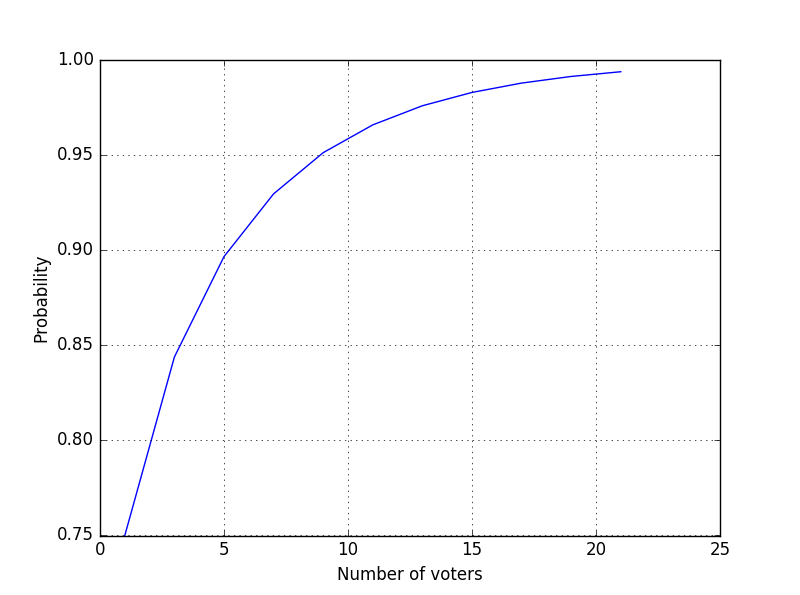
\includegraphics[width=1\textwidth]{condorcet}
\caption{Plot showing the dependency between number of voters and probability result when a single voter probability is 75\%}
\label{fig:condorcet}
\end{center}
\end{figure}


\subsection{Implementation}

For fulfilling goals in the related topic a custom application was written using Python 2.7 programming language. The application contains the following components:
\begin{itemize}
\item Raw data reader - connects to a BCI headset over Bluetooth and reads raw data
\item Preprocessor -  does Short-time Fourier transform of a bulk raw data and determines signal amplitudes for desired frequencies (features)
\item Data storer - stores preprocessed data to a file system (e.g CSV file)
\item Classificator - a machine learning algorithm which teaches classificator and uses it to predict preprocessed a target based on features
\item Voting handler - in case of multi-trial sessions it is used to select the right answer
\item Main application - provides a command-line user interface to select application modes and run necessary components
\end{itemize}

Some of the major components are described in the following subsections.
\begin{figure} [ht]
\begin{center}
\includegraphics[width=1\textwidth]{application}
\caption{Application structure model}
\label{fig:fnCompModel}
\end{center}
\end{figure}

\subsubsection{Raw data reader}

This component is required to poll the Emotiv EPOC headset and store sent data to a temporary buffer. The communication between computer and headset is established over a Bluetooth Smart network through a USB dongle provided from the manufacturer. Emokit\cite{emokit} open-source library with minor changes is used to read the data coming to USB dongle from a headset, decrypt and encode it. Polling is done in an infinite loop. Taking into account sampling frequency of the device - 128 Hz, every ~8 ms a new signal is received from the headset and stored in a queue.

\subsubsection{Preprocessor}

During preprocessing a set of raw samples is converted to a frequency domain representation. To do this the Short Time Fourier Transform is used with a sliding window. Sliding window technique allows to capture more precisely non-constant signals. Sliding window length equals to 1 s with 0.5 s overlapping. These factors increase the number of samples to $2*N-1$ where $N$ is the original number of samples. For example a BCI session with a duration of 1 minute will output 119 samples.

According to Emotiv EPOC specifications\cite{emotiv} 45 Hz is the maximum bandwidth value for the signal. In our implementation we use 1 - 45 Hz for the frequency range.

\subsubsection{Classificator}

Classificator component is responsible for determination of a target (class) from the number of samples given by preprocessor component. Each sample (record) contains amplitudes for all the sensors and different frequencies which makes $14*45=630$ features. In addition to them we add a timestamp and a target name to each record. This records compose a dataset which is fed up to a classificator (machine learning algorithm) to train it. 

Train data could be separated from test data in different ways:

\begin{itemize}
\item Using first majority of samples as train data and other as test data. For example it could be 70\% for train and 30\% for test data.
\item Using cross-validation. This means selecting proportional test data chunks (e.g 20\%) from the whole dataset without overlapping and using the rest of samples as train data. This will result in training several classificators. A classificator with the highest accuracy will be chosen finally.
\end{itemize}

\subsection{Application modes}
\subsubsection{Training mode}
\subsubsection{Testing mode}

\subsection{Targets}
For the targets in the current system two classes were selected: 
\begin{itemize}
\item Relax - the mental task considering a subject to focus sight on a fixation cross and trying to meditate.
\item Excitement - the high performance mental task considering a subject to try focusing on a fixation cross and calculate the mathematical expressions provided by the system.
\end{itemize}

\begin{figure} [H]
\begin{center}
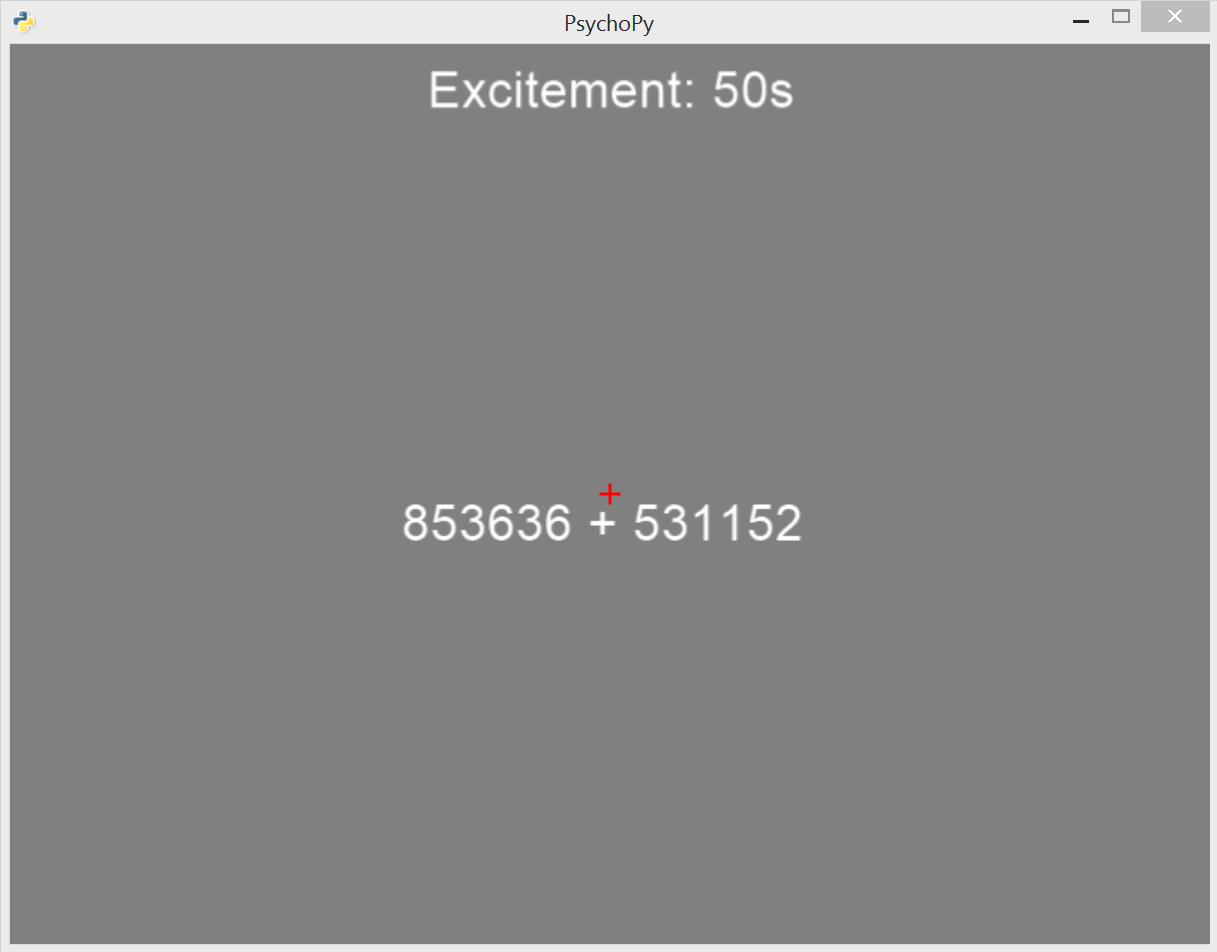
\includegraphics[width=0.7\textwidth]{test_ui}
\caption{A dialog window displaying what a subject sees during a test for both target tasks. A red fixation cross is located at the center of the window}
\label{fig:fnCompModel}
\end{center}
\end{figure}

At the beginning of the classification experiments the motor activity signals were used as targets, upon it was made clear that Excitement and Relax are actually giving better prediction results. The motor activity signals:
\begin{itemize}
\item Left - the motor task considering imaging movement of the left hand.
\item Right - the motor task considering imaging movement of the right hand.
\end{itemize}

The results connected to the motor tasks are also provided in the validation section.

With the several measurements and verifications it was determined that 10 seconds is the suitable measurement session length. Taking into account that every second of measurement produces 18 samples after the short-time Fourier transformation the provided period is containing 180 ($10*18=180$) signal data samples. The classification result from this sample is calculated either using majority or weighted vote.
\newpage
\section{Validation}
\subsection{Motor activity tasks validation}

\subsection{Relax and Excitement tasks validation}
\subsubsection{Majority voting}
\subsubsection{Weighted voting}
\newpage
\section{Discussion}

\newpage
\section{Conclusion}

\newpage
\begin{thebibliography}{9}

\bibitem{bci_jonathan}
Wolpaw JR, Birbaumer N, McFarland DJ, Pfurtscheller G, Vaughan TM.
Brain-computer interfaces for communication and control. Clin Neurophysiol. 2002 
Jun;113(6):767-91. Review.
\bibitem{bci_vidal}
Vidal JJ. Toward direct brain-computer communication. Annu Rev Biophys Bioeng.
1973;2:157-80. Review.
\bibitem{bci_shivangi}
Shivangi Miglanim, Surbhi Gupta.  International Journal of Emerging Research in Management \&Technology
ISSN: 2278-9359 (Volume-2, Issue-8)
Brain Computer Interface. 
August 2013
\bibitem{emotiv}
Emotiv EPOC specifications. https://www.emotiv.com/epoc/
\bibitem{alfahoum_fft}
Al-Fahoum AS, Al-Fraihat AA. Methods of EEG Signal Features Extraction Using Linear Analysis in Frequency and Time-Frequency Domains. ISRN Neuroscience. 2014;2014:730218.
\bibitem{classification_basics}
Pang-Ning Tan, Michael Steinbach, Vipin Kumar. Introduction to Data Mining. March 25, 2006. ch. 4, pp. 146-149.
\bibitem{ml_types}
Russell, Stuart; Norvig, Peter (2003) [1995]. Artificial Intelligence: A Modern Approach (2nd ed.). Prentice Hall. ISBN 978-0137903955
\bibitem{masso}
Madis Masso, Empirical Comparison of Machine Learning Algorithms Based on EEG Data. 2016
\bibitem{breiman_rf}
Breiman, L. Machine Learning (2001) 45: 5. 
\bibitem{collaborative_wang}
Wang, Yijun, and Tzyy-Ping Jung. ``A Collaborative Brain-Computer Interface for Improving Human Performance.'' Ed. Pedro Antonio Valdes-Sosa. PLoS ONE 6.5 (2011): e20422. PMC. Web. 10 Nov. 2016.
\bibitem{emokit}
Emokit SDK. https://github.com/openyou/emokit
\end{thebibliography}

%\bibliography{bachelor-thesis}

\appendix

\begin{figure} [H]
\begin{center}
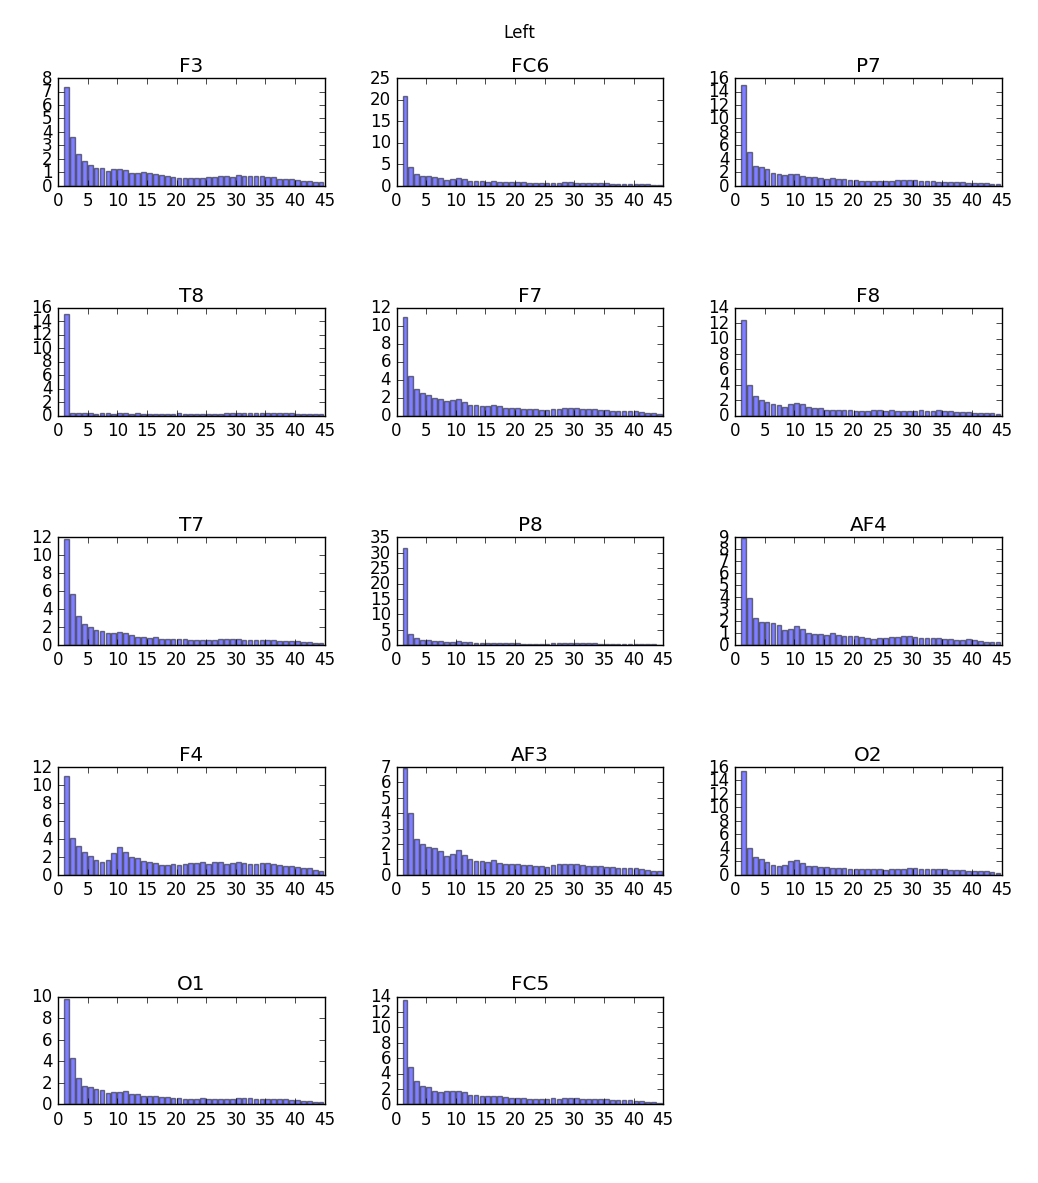
\includegraphics[width=1\textwidth]{left_amplitudes}
\caption{A sample frequency domain plot while concentrating on "Left" target. Vertical axis is measured in Hz. Horizontal in $\mu$V.}
\end{center}
\end{figure}

\pagebreak
\section*{\small Non-exclusive licence to reproduce thesis and make thesis public}


I, Jevgeni Savostkin (date of birth: 13th of March 1990),

\begin{tabbing}
\= Xiii\=\kill
\>1. \> herewith grant the University of Tartu a free permit (non-exclusive licence) to:\\\\ 

\>1.1\> 
\begin{minipage}[t]{14.2cm}
reproduce, for the purpose of preservation and making available to the public, including for addition to the DSpace digital archives until expiry of the term of validity of the copyright, and
\end{minipage}
\\\\
\>1.2 
\begin{minipage}[t]{14.2cm}
make available to the public via the web environment of the University of Tartu, including via the DSpace digital archives until expiry of the term of validity of the copyright,\\ 

Improving accuracy of brain-computer interface with multiple trials\\   

supervised by Ilya Kuzovkin and Raul Vicente

\end{minipage}\\\\ 
\>2. \>I am aware of the fact that the author retains these rights.\\\\
\>3. \>
\begin{minipage}[t]{14.2cm}
I certify that granting the non-exclusive licence does not infringe the intellectual property rights or rights arising from the Personal Data Protection Act. 
\end{minipage}\\
\end{tabbing}

\noindent
Tartu, dd.mm.yyyy


\end{document}
